% !TEX TS-program = xelatex
% !TEX encoding = UTF-8 Unicode
% !Mode:: "TeX:UTF-8"
\documentclass[bachelor, printoneside]{seuthesis} % 本科
% \documentclass[master]{seuthesis} % 硕士
% \documentclass[doctor]{seuthesis} % 博士
% \documentclass[engineering]{seuthesis} % 工程硕士
\usepackage{CJK,CJKnumb}
\usepackage{amsmath}
\usepackage{amsfonts} 
\usepackage{bm} 
\usepackage[linesnumbered,ruled,vlined]{algorithm2e}
\usepackage{multirow}
\usepackage{hyperref}

% 导言区
\begin{document}
\categorynumber{000}    % 分类采用《中国图书资料分类法》
\UDC{000}               %《国际十进分类法UDC》的类号2
\secretlevel{公开}        % 学位论文密级分为"公开"、"内部"、"秘密"和"机密"四种
\studentid{09013119}    % 学号要完整,前面的零不能省略。

\title{基于多知识库的表格实体链接研究}{副标题}{Entity Linking in Web Tables with Multiple Linked Knowledge Bases}{subtitle}
\author{严晟嘉}{Shengjia Yan}
\advisor{李慧颖}{教授}{Huiying Li}{Prof.}
\coadvisor{漆桂林}{教授}{Guilin Qi}{Prof.}

% \degree{工学硕士} % 详细学位名称
\major[12em]{计算机科学与技术}
\defenddate{答辩日期}
\authorizedate{学位授予日期}
\department{计算机科学与工程}{Computer Science \& Engineering}
\duration{2017.01 — \ 2017.06}
\address{东南大学九龙湖校区}
\thanks{}
\maketitle

% 中文摘要
\begin{abstract}{实体链接,Web表格,多知识库}
在当今的万维网上包含着超大规模的蕴含丰富价值的关系型数据,而这些关系型数据大多以 HTML 表格 (也就是 Web 表格) 的形式呈现。
抽取 Web 表格中的语义来生产机器可以理解的知识如今已经成为了一个热门的研究领域。
从 Web 表格中抽取出丰富且高质量的语义信息是一个充满挑战和价值的任务,其中关键一步就是实体链接 (Entity Linking),其目的在于建立表格中的字符串指称 (Mention) 到知识库中的相应的参考实体 (Entity) 的链接。\par

目前大部分的实体链接都是使用单个特定的跨领域知识库来作为实体数据的来源。
但由于单个知识库中的实体数量有限且对实体的覆盖范围不广,从而导致单知识库实体链接中实体缺失和链接错误的问题常有发生。
本文提出了两个通用的表格实体链接的新方法。
与先前的工作不同的是,这两个方法都使用多知识库而不是单知识库作为实体数据的来源,来提升表格实体链接的质量。\par

方法一是一个``两步走''的方法,首先将一个基于图模型的随机游走算法应用于单知识库的表格实体链接,然后使用多知识库间已有的和新学习到的``sameAs''关系来提升前一步中实体链接结果的质量。
方法二融合了方法一中的两步,修改了方法一中图模型中的节点定义,直接将多知识库间已有的和新学习到的``sameAs''关系融合进了图模型,从而实现了一步到位的效果。\par

我设计了一些对比实验来比较本文提出的两个方法与目前最先进的实体链接系统 (TabEL, LIEGE) 的效果差异。
所有实验都是在基于 Zhishi.me 人工标注的 Web 表格上进行的,Zhishi.me 涵盖了三个最大的中文百科知识库:百度百科,互动百科和中文维基百科。
实验表明,文中提出的两个方法在准确率、召回率、F1 值等评价指标上表现得都很不错。
除此之外,我在实体消岐时引入了更多的有效的特征,还增加了一些有意义的功能,比如``sameAs''关系的学习。
实验中用到的已人工标注的表格语料库和算法的实现代码都是开放的,供未来的研究工作使用。
\end{abstract}

% 英文摘要
\begin{englishabstract}{Entity Linking, Web Tables, Multiple Linked Knowledge Bases}
The World-Wide Web contains a huge scale of valuable relational data, which are embedded in HTML tables (i.e. Web tables).
It's a challenging and valuable task that extracting abundant and high-quality semantics of Web tables is.
A key step in extracting the semantics of Web tables is Entity Linking (EL), which aims to map the string mentions in table cells to their referent entities in a Knowledge Base (KB).\par

At present most entity linking researches use single cross-domain KBs as source of entities.
However, the quantity of entities and the coverage in a single KB is limited.
Thus, the issues of entity absence and linking error often appear in the process of EL in a single KB.
In this paper, I present two new approaches for EL in Web tables.
Different from previous work, the proposed approaches replace a single KB with multiple linked KBs as the sources of entities to improve the quality of EL.

Approach One is a two-step method.
I first apply a random walk algorithm based on a general probabilistic graphical model to EL in Web tables with each single KB.
Then, I leverage the existing and newly learned ``sameAs'' relations between the entities from different KBs to help improve the results of EL in the first step.
Approach Two merges two steps from Approach One.
I modify node definitions in the probabilistic graphical model in Approach One and directly add the ``sameAs'' relations between the entities from different KBs into the model.\par

Some comparison experiments are designed to compare the effect of my approaches proposed in this paper with the state-of-the-art table’s EL systems (TabEL, LIEGE).
All experiments are conducted on the sampled Web tables with Zhishi.me, which consists of three biggest linked Chinese encyclopedic KBs: Baidubaike, Hudongbaike and Zhwiki.
The experimental results show that my approaches have a good performence in different evaluation metrics, such as precision, recall and F1 value.
Besides, I adds some meaningful functions, such as iterative learning between EL and ``sameAs'' relations.
I also make my manually annotated table corpus and the code of the approaches publicly available for future work.
\end{englishabstract}

% 目录
\tableofcontents

% 术语表
% \begin{terminology}

\begin{table}[h]
%\Large
\begin{tabular}{|>{\LARGE}m{0.2\textwidth}<{\centering}|m{0.8\textwidth}|}
\hline
\normalsize \hspace*{\stretch{1}}术语\hspace*{\stretch{1}} & \hspace*{\stretch{1}}含义\hspace*{\stretch{1}} \\ 
\hline
a & 如同汉字起源于象形,拉丁字母表中的每个字母一开始都是描摹某种动物或物体形状的图画\\
\hline
b & 和A一样,字母B也可以追溯到古代腓尼基。在腓尼基字母表中B叫beth,代表房屋,在希伯来语中B也叫beth,也含房屋之意。\\
\hline
c& 字母C在腓尼基人的文字中叫gimel,代表骆驼。它在字母表中的排列顺序和希腊字母Γ(gamma)相同,实际上其字形是从后者演变而来的。C在罗马数字中表示100。\\
\hline
d&D在古时是描摹拱门或门的形状而成的象形符号,在古代腓尼基语和希伯来语中叫做daleth,是“门”的意思,相当于希腊字母Δ(delta)。\\
\hline
\end{tabular}
%\caption{my table}
\end{table}

\end{terminology}

% 开始正文
\begin{Main}

\chapter{绪论}

\section{研究动机}
如今 Web 上的内容每天都在以指数级的速度增长\cite{limaye2010annotating},这也使得 Web 近年来成为世界上最大的数据集散地之一。
据估计 Web 上有超过141亿张表格,其中1.54亿张表格包含关系型数据并且仅 Wikipedia 就是大约160万关系型表格的来源。
可见Web 表格,换句话说是 Web 上的 HTML 表格,是关系型数据的一个重要来源和信息抽取 (Information Extraction) 系统的一个重要输入。
与普通文本不同,单张关系型表格就包含一系列高质量的关系实体并且在表格的表头中包含与实体相关的元数据。
Web 上包含关系型数据的表格中蕴含的巨大财富和价值使得表格的语义解释 (Semantic Interpretation),也就是将 Web 表格转换成机器能够理解的知识这一任务成为热门的研究领域。\par

另一方面,诸如维基百科等知识共享社区的蓬勃发展和信息抽取技术的进步已经促成了大规模机器可读知识库的自动化建设。
目前世界上已经出现了上百个领域不同、规模不一的知识库 (Knowledge Base) 并且它们的规模每天都在飞速增长。知识库中包含着整个世界的实体,实体的语义类别及其相互关系的丰富信息。
这样典型的例子包括 YAGO\cite{suchanek2007yago},DBpedia\cite{auer2007dbpedia} 和 Freebase\cite{bollacker2008freebase}。
在中文知识库中较有影响力的就是由上海交通大学和东南大学共同建立的 Zhishi.me\cite{niu2011zhishi}。\par

Web 上虽然蕴含着许多有价值的数据,但更多的却是各种原始并且充斥着噪声的数据,其中有些甚至是错误的。
这些数据大都是以自然语言的形式存在,然而由于自然语言表达的多样性与歧义性,使得它们很难被计算机直接处理或者理解。
面对如此规模庞大而嘈杂的数据,信息过载的现象每天都在发生。
信息过载意味着在找到想要的有用的信息之前,需要处理大量的无用数据,计算机获取有效信息的效率常常受到限制。
为了减轻信息过载带来的负面影响以及处理自然语言的多样性问题和歧义性问题,语义网 (Semantic Web) 的概念应运而生,旨在对现有万维网上的文档进行元数据 (Meta Data) 标注,使计算机能够理解词语和概念以及它们之间的逻辑关系。
将 Web 数据与知识库链接起来是非常有利于标注 Web 上的大规模数据的,并且有助于实现语义网的愿景\cite{berners2001semantic}。
许多为了解释说明 Web 表格内含的语义的研究工作\cite{limaye2010annotating}\cite{hignette2009fuzzy}\cite{mulwad2013semantic}\cite{munoz2014using}\cite{syed2010exploiting}\cite{venetis2011recovering}是将其内容标注成 RDF 三元组。
这种语义标注 (Semantic Annotation) 的关键一步就是实体链接 (Entity Linking),将出现在 Web 表格单元格中的字符串指称 (Mention) 链接到其在给定知识库中对应的参考实体 (Entity)。\par

实体链接技术的发展可以带动许多不同的应用的发展,比如知识库补全,自然语言问答系统和语义搜索系统。
随着社会的发展,新的知识被创造出来并以数据的形式表现在 Web 上。
因此,利用这些新知识扩充现有的知识库显得越发重要。
然而,为了将这些新知识插入到现有知识库中,会不可避免地需要一个系统,来将字符串指称,也就是与已抽取出的知识相关联的指称,链接到知识库中的相应实体。
例如,自然语言问答系统依靠它们支持的知识库来回答用户的问题。
为了回答``苹果公司创始人史蒂夫·乔布斯的诞生日期是哪天''这个问题,该系统应首先利用实体链接技术将查询语句中的``史蒂夫·乔布斯''映射到美国企业家,而不是美国传记电影,
然后从知识库中直接取回名为``史蒂夫·乔布斯''的出生日期。
除此之外,实体链接对数据集成很有帮助,可以将不同页面、文档和站点上的实体信息进行集成。
可见,Web 表格上的实体链接技术很有价值并且拥有广阔的应用前景。\par


\section{研究现状}

在本节中,我会回顾一些在 Web 表格上进行语义标注的相关研究工作,它们通常会处理三个任务:实体链接 (Entity Linking),列类型推理 (Column Type Inference) 以及关系抽取 (Relation Extraction)。 
在 Cafarella 等人\cite{cafarella2008webtables}报告说,有超过1.5亿个 Web 表格内嵌有高质量的关系型数据,许多研究人员意识到 Web 表格是许多应用的重要数据来源,比如信息抽取和结构化数据搜索。 
因此,与 Web 表格的语义标注相关的各种研究工作如雨后春笋般涌现出来。\par

Hignette 等人\cite{hignette2009fuzzy}提出了一种聚合的方法,使用给定本体中的词汇来标注 Web 表格中的内容。
它首先标注单元格,然后标注列的类型,最后标注列之间的关系。
与之相似的,Syed 等人\cite{syed2010exploiting}提出了一种管道方法,其首先进行列类型推理,然后将单元格的值链接到给定的知识库中的实体,最后选择列之间合适的关系。
Zhang \cite{zhang2014towards}设计了一个名为 TableMiner 的工具来标注 Web 表格。
TableMiner 只专注于列类型推理和实体链接,并不能从 Web 表格中抽取关系。
之后,Zhang \cite{zhang2014learning}又提出了一些策略来改进 TableMiner。 
Limaye 等人\cite{limaye2010annotating}和 Mulwad 等人\cite{mulwad2013semantic}提出了两种方法,可以分别对 Web 表格上的实体链接,列类型推理和关系抽取任务联合建模。
我的方法和这些研究工作之间的主要区别在于它不依赖任何特定的信息来完成实体链接的任务,例如 Web 表格的表头和标题,知识库中的实体类型和网页中的语义标记等等。\par

还有一些在特定场景下对 Web 表格进行语义标注的研究工作是没有实体链接的步骤的。
在 Venetis 等人\cite{venetis2011recovering}的研究工作中,他们的方法是弱化实体链接的影响,直接进行列类型推理,并且通过大规模的关系数据库 (Relation Databases) 中不同模式的出现频率来确定 Web 表格中的关系,这些关系数据库都是由网页构建的,但通常不对大部分研究人员开放。
此外,Munoz 等人\cite{munoz2014using}提出了一种从维基百科表格中挖掘 RDF 三元组的方法。
在这项研究中,他们能够通过内部链接和文章标题直接识别出维基百科中的实体。\par

跟我的方法最相近的研究工作是 Bhagavatula等人\cite{bhagavatula2015tabel} 和 Shen 等人\cite{shen2012liege}的研究工作。
Shen 等人\cite{shen2012liege}尝试将形如列表 (List-like) 的 Web 表格 (表格有多行但只有一列) 中的字符串指称链接到给定知识库中的实体。
Bhagavatula 等人\cite{bhagavatula2015tabel}提出了 TabEL,一个表格实体链接系统,它使用集体分类技术来对 Web 表格中的所有指称进行联合消岐 (Entity Disambiguation)。
这两个研究工作都不使用任何特定信息来进行实体链接,并且可以应用于任何知识库。
在本文中,为了提高 Web 表格中的实体链接的质量,我专注于在多个相互有链接关系的知识库下的实体链接而不是单个知识库下的实体链接。\par


\section{本文贡献}\label{contribution}

之前的 Web 表格实体链接研究中主要存在两个问题。
1) 许多研究工作\cite{limaye2010annotating}\cite{hignette2009fuzzy}\cite{mulwad2013semantic}\cite{syed2010exploiting}\cite{zhang2014towards}\cite{zhang2014learning}都非常依赖于基于特定信息的特征,
比如 Web 表格的表头 (e.g. ``电影'',``导演''等等。在图~\ref{el} 中表格的第一行中出现),目标知识库中的实体类型以及其他的一些特定信息。
假如我们要处理的 Web 表格中没有这样的表头信息抑或是给定的知识库中没有实体类型的信息,那么很显然前面提及的那些方法的效果会很有限。
2) 现在大部分实体链接的方法\cite{limaye2010annotating}\cite{hignette2009fuzzy}\cite{syed2010exploiting}\cite{zhang2014towards}\cite{zhang2014learning}\cite{shen2012liege}\cite{bhagavatula2015tabel}都只考虑将 Web 表格单元格中的字符串指称链接到单一知识库,但是每个知识库中的实体数量都是有限的,单一知识库无法保证在做 Web 表格上的实体链接的时候对实体有一个很好的覆盖度。
单知识库上的实体链接常常会出现实体缺失的状况。这个问题在这篇论文\cite{pereira2014entity}中的自然语言文本上实体链接的过程中也有体现。\par

为了克服上述问题,在我的毕业设计``基于多知识库的表格实体链接研究''中,我提出了两个新的通用的方法来做基于多知识库的 Web 表格实体链接。
1) 方法一中包含两个步骤。第一步是将一个不依赖于任何特定信息的基于图模型 (Probabilistic Graph Model) 的算法用来做 Web 表格与每个单知识库的实体链接。
然后在第二步中,我提出了三个启发式规则,利用来自不同知识库的实体之间的已存在的和新学习的 ``sameAs'' 关系,以提高第一步的实体链接结果的质量。
第二步不仅可以减少单知识库实体链接产生的错误,还可以提高实体链接结果的覆盖范围。
2) 方法二基于一种融合的思想,尝试用一个统一的图模型来表示 Web 表格中的字符串指称和来自多知识库的实体信息,然后在这个图模型上进行随机游走 (Random Walk),直接得到实体链接的结果。
简单的说,方法二融合了方法一中的两步,将多知识库间的 ``sameAs'' 关系加进了图模型,
同时也舍弃了方法一中的启发式规则,毕竟启发式规则是基于直觉和经验而定,在实际操作中有可能会因为多知识库间 ``sameAs'' 关系的缺失而舍弃一些非常有价值的实体链接结果,方法二规避了这些风险。
在实验中,我将一些 Web 表格样本中的字符串指称与 Zhishi.me\cite{niu2011zhishi} 中的实体进行链接,Zhishi.me 是最大的中文链接开放知识库,如图~\ref{zhishime_link} 所示,其由三个相互链接的中文在线百科知识库组成:中文维基百科\footnote{\url{https://zh.wikipedia.org}},百度百科\footnote{\url{http://baike.baidu.com}}和互动百科\footnote{\url{http://www.baike.com}}。

针对本文中的两个方法,设计了一些对比试验来将它们和目前最先进的实体链接系统 (即 TabEL\cite{bhagavatula2015tabel} 和 LIEGE\cite{shen2012liege}) 进行各方面的比较。
实验结果表明,本文中提出的方法在 MRR(即 Mean Reciprocal Rank\footnote{\url{https://en.wikipedia.org/wiki/Mean_reciprocal_rank}} 平均倒数排名),准确率,召回率和 F1 值等评价指标上都表现得很不错。
实验中用到的表格语料库和算法的实现代码\footnote{\url{https://github.com/yanshengjia/link}}都是公开的,人工标注实体的表格数据同样也对未来的表格实体链接研究者开放。\par

% Fig
\begin{figure}[htbp]
\centering
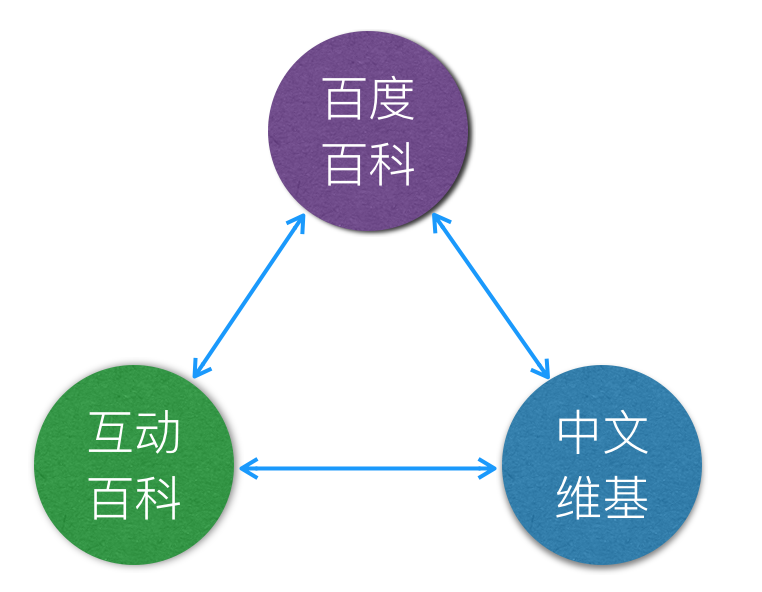
\includegraphics[width=0.4\textwidth]{img/zhishime_link}
\caption{Zhishi.me 由三个相互链接的知识库组成}
\label{zhishime_link}
\end{figure}

总而言之,本文的主要贡献在于:
\begin{enumerate}[1.]
  \item 提出了一个两阶段的基于多知识库的表格实体链接方法 (即方法一),并在实验中体现其比基于单一知识库的实体链接方法的优越性。该方法不依赖表格和知识库中的特定信息,而是建立了一个通用的图模型并使用随机游走算法来进行实体的迭代消岐。
  \item 提出了一个融合的支持多知识库的表格实体链接方法 (即方法二),其融合了方法一中的两步,规避了方法一中的启发式规则带来的风险,整个方法都是在一个统一的图模型上运行,一步到位得得出链接结果。
  \item 设计了一些对比试验,将本文提出的两个方法,TabEL\cite{bhagavatula2015tabel} 和 LIEGE\cite{shen2012liege} 在链接准确率、召回率、F1 值和 MRR 值上进行比较,从而验证本文提出的两个方法的效果。
  \item 在实体消岐时相较于以前的方法使用了很多十分具有价值的特征,比如字符串相似度特征、上下文相似度特征、同义词特征、三元组关系特征、知识库实体的消岐义特征等等。
  \item 添加了一些很有意义的功能,比如``sameAs'' 关系的学习。多知识库间的 ``sameAs'' 关系往往是不完备的,利用实体链接的结果可以与``sameAs''关系进行迭代学习,另外也可以通过监督学习分类器 SVM\cite{tong2001support} 进行``sameAs''关系的学习。
\end{enumerate}

本文的各章节内容是这样分配的:第一章是绪论的,介绍了我的毕设项目的研究动机、相关研究工作以及本文的主要贡献;
第二章从背景知识的角度出发阐述了基于多知识库的实体链接技术的方方面面,包括任务目标、关键挑战以及一般链接流程;
第三章详细介绍了我的毕设研究中提出的两个方法的思想以及相关模型;
第四章从算法具体实现的角度切入,以一个工程师的身份讲述实现细节;
第五章是实验与评估,详述了整个实验流程,将本文中的两个方法与 TabEL\cite{bhagavatula2015tabel} 和 LIEGE\cite{shen2012liege} 在不同评价指标上进行对比并分析;
第六章也就是最后一章总结了全文,并展望了未来工作。













\chapter{基于多知识库的表格实体链接}

\section{任务描述}


\section{关键挑战}



\section{链接流程}



\section{本章小结}
\chapter{描述}\label{description}

由前两章内容可知,实体链接的一般流程包括指称识别、候选实体生成和实体消岐。
其中实体消岐的部分最有挑战也最为关键。
整个实体消岐的过程在有些文献\cite{shen2015entity}中也称为``候选实体排名'',对字符串指称的候选实体进行排名,最终排名最高的实体被选为指称的对应参考实体。
这个排名的过程与网页排名算法 PageRank\cite{page1999pagerank} 类似。
由表格的特点可知,单元格之间往往存在一定的语义相关性,这种语义相关性让两个单元格中的字符串指称关联在一起。
在知识库中,不同的实体之间也可能存在一定的语义相关性,同样,指称和实体之间也是可能语义相关的。
相互关联的字符串指称的链接结果可能会互相影响,为了充分利用这些语义相关性,马尔科夫链模型\cite{stewart1994introduction}是一个好选择。
马尔科夫链可以用来捕捉指称与实体、实体与实体之间的语义相关性,从而提高实体链接的质量。
在我的两个方法中,实体消岐的算法都运用了马尔科夫链模型和一个个性化的 PageRank 算法\cite{haveliwala2003topic}\cite{langville2011google},而 PageRank 算法建立在随机游走模型上\cite{haveliwala2003topic},并且随机游走就是一种马尔科夫链的例子,所以我的方法其实就是在马尔科夫链模型上进行随机游走。
马尔科夫链可以用图表示,因此毕设中的两个方法也可以称为是基于图的随机游走算法。
在本章中,我会先介绍马尔科夫链模型和随机游走模型,然后详细地描述两个方法的细节。


\section{马尔可夫链}
马尔可夫链,为状态空间中经过从一个状态到另一个状态的转换的随机过程。
该过程要求具备``无记忆''的性质:下一状态的概率分布只能由当前状态决定,在时间序列中它前面的事件均与之无关。
这种``无记忆性''称为马尔可夫性质。
图~\ref{markov_chain} 中即为一个马尔科夫链的例子。
在马尔可夫链的每一步,根据概率分布,可以从一个状态变到另一个状态,也可以保持当前状态。
状态的改变叫做转移,与不同的状态改变相关的概率叫做转移概率。
随机漫步就是马尔可夫链的例子。
随机漫步中每一步的状态是在图形中的点,每一步可以移动到任何一个相邻的点,在这里移动到每一个点的概率都是相同的 (无论之前漫步路径是如何的)。\par

% Fig 
\begin{figure}[htbp]
\centering
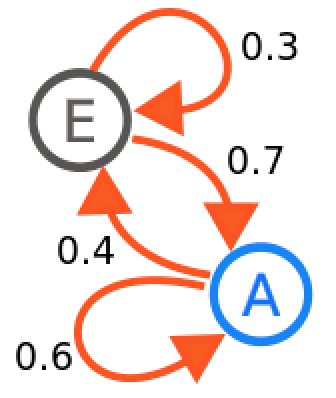
\includegraphics[width=0.15\textwidth]{img/markov_chain}
\caption{一个具有两个转换状态的马尔可夫链}
\label{markov_chain}
\end{figure}

若状态空间是有限的,则马尔科夫链的转移概率分布可以矩阵表示,该矩阵称为转移矩阵,记为 $\bm{P}$,在后文中迭代概率繁殖中也称为概率转移矩阵。
如果 $\bm{P}$ 是一步转移矩阵,$\bm{P}^k$ 就是 $k$ 步转移后的转移矩阵。
由马尔科夫链\footnote{\url{https://en.wikipedia.org/wiki/Markov_chain}}在有限状态空间内的性质\cite{tauchen1986finite}可知,如果转移矩阵 $\bm{P}$ 不可约且非周期,则 $\bm{P}$ 会收敛到一个独立的稳态分布 $\bm{\pi}$。
用公式表示如下:
\begin{equation}
	\lim_{k \rightarrow \infty} \bm{P}^k = \bm{1} \bm{\pi}
\label{pk}
\end{equation}
其中 $\bm{1}$ 是一个列向量每个元素都为1。
还有一个关于马尔科夫链的重要性质是一个正转移矩阵 (矩阵中每个元素都为正) 是不可约和非周期的。
这些性质都是~\ref{single} 节中迭代概率传播算法的理论基础。
它们保证了在实体消岐图上运行随机游走算法能够在有限次迭代内达到收敛。


\section{随机游走}
随机游走,是一种数学统计模型,由一连串的轨迹所组成,其中每一次都是随机的。
它能用来表示不规则的变动形式,如同一个人酒后乱步,所形成的随机过程记录。
通常,可以假设随机游走是以马尔可夫链或马可夫过程的形式出现。
在图~\ref{random_walk} 中是一个一维随机游走的例子。
PageRank\cite{page1999pagerank} 算法可以用随机游走模型来解释\cite{haveliwala2003topic}。
PageRank 通过 Web 上的超链接关系来确定一个页面的等级,用于计算网页的相关性和重要性。

% Fig 
\begin{figure}[htbp]
\centering
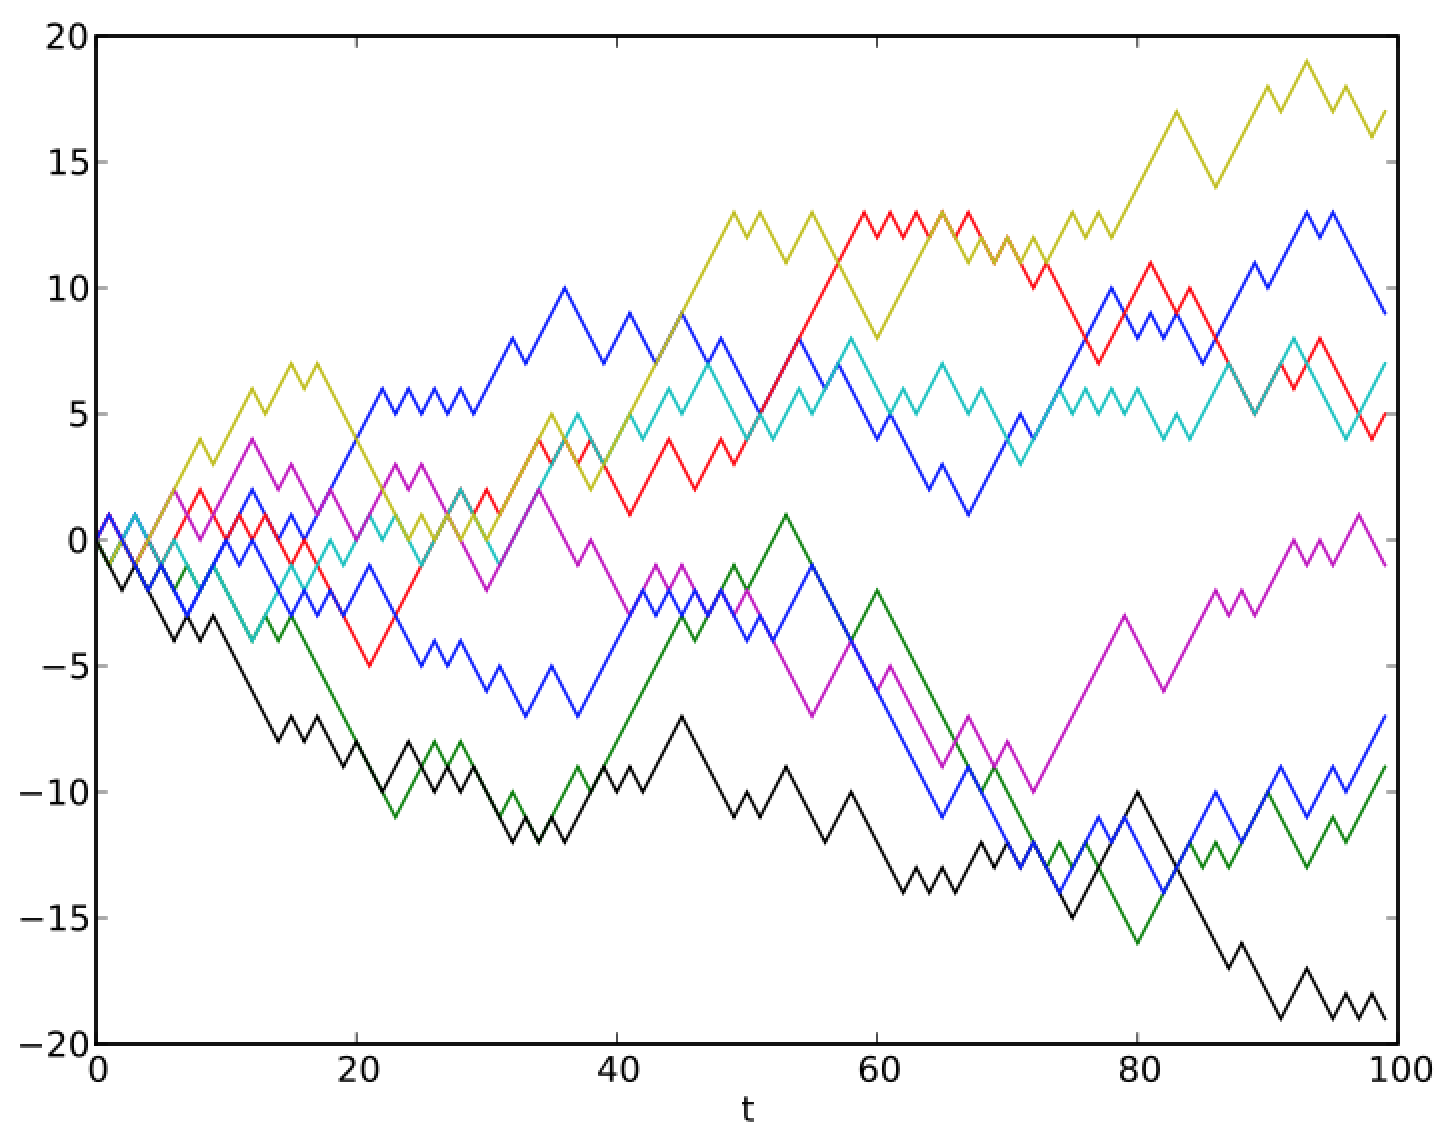
\includegraphics[width=0.35\textwidth]{img/random_walk}
\caption{一维的随机游走。纵轴表示当前的位置,横轴表示时间步数。}
\label{random_walk}
\end{figure}


\section{方法一: 两步走}\label{approach1}

方法一包含两个主要的步骤:首先使用各个单知识库进行实体链接,然后运行多知识库间的 ``sameAs'' 关系来优化单知识库的链接结果。

% Fig 
\begin{figure}[htbp]
\centering
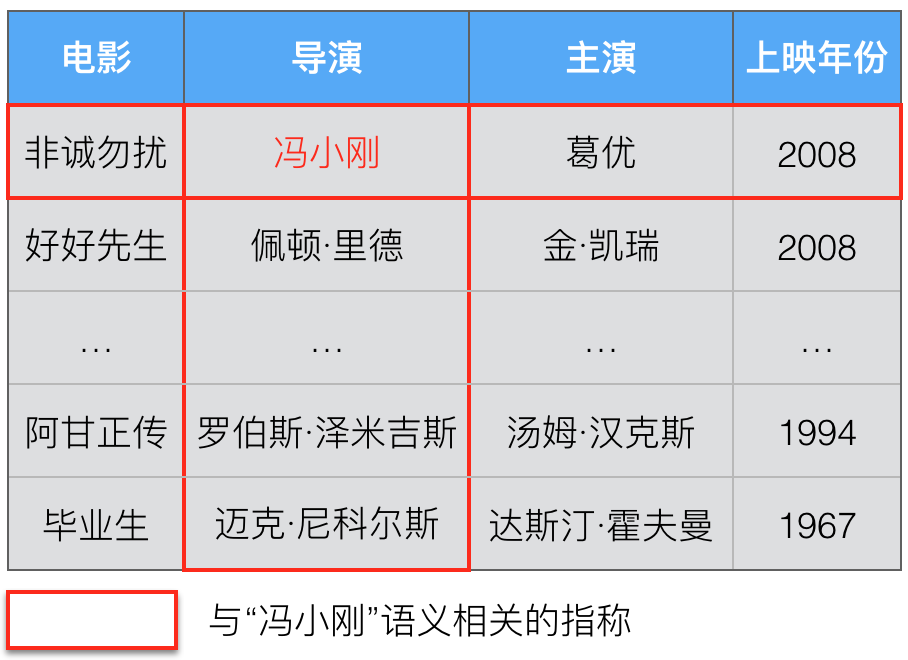
\includegraphics[width=0.6\textwidth]{img/table}
\caption{一个表格同行同列中的指称具有语义相关性的示例}
\label{table}
\end{figure}

\subsection{单知识库表格实体链接}\label{single}

\noindent\textbf{指称识别} \ 
任何实体链接系统的第一步是识别出潜在的字符串指称,它们能够被链接到知识库中的参考实体。
给定来自输入的表格中每个单元格的文本内容,$t_q$,系统将 $t_q$ 中满足一定条件的最长的短语 $s$ 识别为潜在的指称。
这个条件就是对于某些实体 $e$,字符串 $s$ 能链接到该实体的概率 $P(e|s)$ 非零。
如果 $s$ 的长度小于 $t_q$ 的长度,系统会在 $s$ 之后发现长度最长的短语,并以此类推。
例如,对于一个单元格的文本 ``习近平 \& 彭丽媛'',系统会识别出到两个潜在的指称:一个是``习近平'',另一个是``彭丽媛''。\newline


\noindent\textbf{候选实体生成} \ 
对于表格单元格中的每个字符串指称,首先需要从给定的海量的知识库实体中找出一些可能成为该指称参考实体的实体,来缩小实体链接的范围。
这样的实体称为字符串指称的候选实体。这样的过程叫做生成候选实体。
我讲每个指称分割到单词级别,所以每个指称能被表示为一个单词集合。
如果给定知识库中的一个实体 $e$ 或者 $e$ 在 BabelNet\cite{navigli2010babelnet} (一个全网域多语种同义词辞典) 中的一个同义词包含某个指称 $m$ 的分割单词集合中的至少一个单词,那么实体 $e$ 就被认为是指称 $m$ 的一个候选参考实体。
举个例子,字符串指称``苹果''有这样的一些候选实体:``苹果'',``苹果派'',``苹果 [水果]'',``苹果 [智能手机品牌]''。
候选实体生成的结果就是每个指称都可能指向一个候选实体集合。
在实际操作过程中,除了指称与实体的包含关系,我还考虑了二者之间的字符串相似度 (计算公式在后面会提到),设置了一个字符串相似度的阈值。
一般来说,与指称的字符串相似度很低的实体,很有可能表示的是跟指称完全不同的事物,即便它们有包含关系。
所以如果实体 $e$ 和指称 $m$ 的字符串相似度低于阈值,即使 $e$ 包含 $m$,也不将该实体 $e$ 添加进 $m$ 的候选实体集合。
比如,对于指称``苹果'',在知识库中有这样的一个实体``苹果红蜘蛛'',显然二者不可能相链接,虽然这个实体里包含了``苹果''二字,但是由于二者的字符串相似度太低,这样的实体就被剔除了。
\newline

\noindent\textbf{实体消岐} \ 
一个指称的候选实体集合可能是空集,也可能包含一个或多个候选实体。
当候选实体集合是空集的时候,那么这个指称是不可链接的,给它打上``NIL''标签。
当候选实体集合中包含多个候选实体的时候,哪个候选实体最有可能成为字符串指称的对应参考实体就成了需要考虑的问题。
从指称的候选实体集合中挑选一个最合适的实体作为指称在给定知识库中的对应参考实体就是实体消岐的目标。
就像图~\ref{table} 中所示,可以发现在同一行或者同一列的指称很可能是语义相关的。
换句话中,出现在同一个 Web 表格中的任意两个指称之间可能存在着一些潜在的联系。
因此,我选择使用一个基于图的随机游走算法来对一个表格中的所有指称进行联合消岐。
实体消岐分为三个子步骤:
\begin{enumerate}[a)]
\item 首先,对于每张给定的表格,建立一个实体消岐图 (Entity Disambiguation Graph),这张图只使用表格中的指称和它们的候选实体作为图中的结点。构建实体消岐图的过程即为将表格中的指称和其候选实体建模成马尔科夫链的过程。
\item 然后,在每个构筑好的实体消岐图上,计算每个指称的初始权重值用于联合消岐,同时将不同结点间的语义相关度计算出来作为实体链接影响因子 (EL Impact Factors) 来决定到底哪个实体是给定的指称的对应参考实体。
\item 最后,计算实体消岐图的概率转移矩阵并运行随机游走算法,具体来说,就是使用实体链接影响因子进行迭代概率传播 (Iterative Probability Propagation),直到实体结点上的概率收敛,这里的迭代概率传播中的``概率''指的是每个实体结点上的概率,它代表该实体成为给定指称的对应参考实体的概率,最后基于这些实体结点上的概率来得到最终的实体链接结果,指称结点的候选实体结点中概率最高的结点胜出成为指称的对应参考实体。
\end{enumerate}


\noindent\newline 在接下来的部分中,我会讲述这三个子步骤的来龙去脉。

a) \textbf{构建实体消岐图} \ 
对于每张给定的表格,建立一张实体消岐图 (Entity Disambiguation Graph),其包含两种类型的结点和两种类型的边,解释如下:
\begin{itemize}
  \item[$\bullet$] \textbf{指称结点}: 这些结点指的是 Web 表格中的字符串指称
  \item[$\bullet$] \textbf{实体结点}: 这些结点表示指称在给定知识库中的候选参考实体
  \item[$\bullet$] \textbf{指称-实体边}: 一条指称-实体边是一个指称和其候选参考实体集合中的一个实体之间的无向边
  \item[$\bullet$] \textbf{实体-实体边}: 一条实体-实体边是实体之间的无向边
\end{itemize}

一个构建好的实体消岐图的例子在图~\ref{edg} 中展示。
因为论文纸张空间所限,这里只画出了图~\ref{table} 中 Web 表格的实体消岐图的一部分,许多结点和边在图~\ref{edg} 中并没有显示。
每个指称和其候选实体集合中的每个实体间都有一条指称-实体边相连接。
比如指称``非诚勿扰''与它的2个候选实体``非诚勿扰 [电影]''、``非诚勿扰 [相亲节目]''之间都有指称-实体边相连接。
实体-实体边应该在图中所有实体结点间创建。
实体消岐图中的边是无向的,其实也可以理解为双向的,这在之后的迭代概率传播中概率转移矩阵的计算中会提到。
由实体消岐图的结构可知,一个指称结点如果是``NIL''的,那么它不与任何实体结点相连,换句话说,它没有任何相邻的结点。
在这里,两个结点通过一条边直接相连,那么我称这样的两个结点是``相邻''的。
一个指称结点的候选实体集合如果非空,那么它可能有一个或者多个相邻的实体结点。
而一个实体结点则与其所在的实体消岐图的所有其他实体结点相邻,与且仅与一个指称结点相邻,并且该实体结点是这个指称结点的候选实体之一。
需要额外说明的是,如果有两个指称结点的候选实体集合中有相同的知识库实体,在实体消岐图中建立的是两个不同的实体结点,即使它们代表的是同一个实体,而不是只建立一个实体结点。
构建实体消岐图的过程也就是将一张表格中的所有指称和其候选实体建模成一个马尔科夫链的过程。
\newline

% Fig 
\begin{figure}[htbp]
\centering
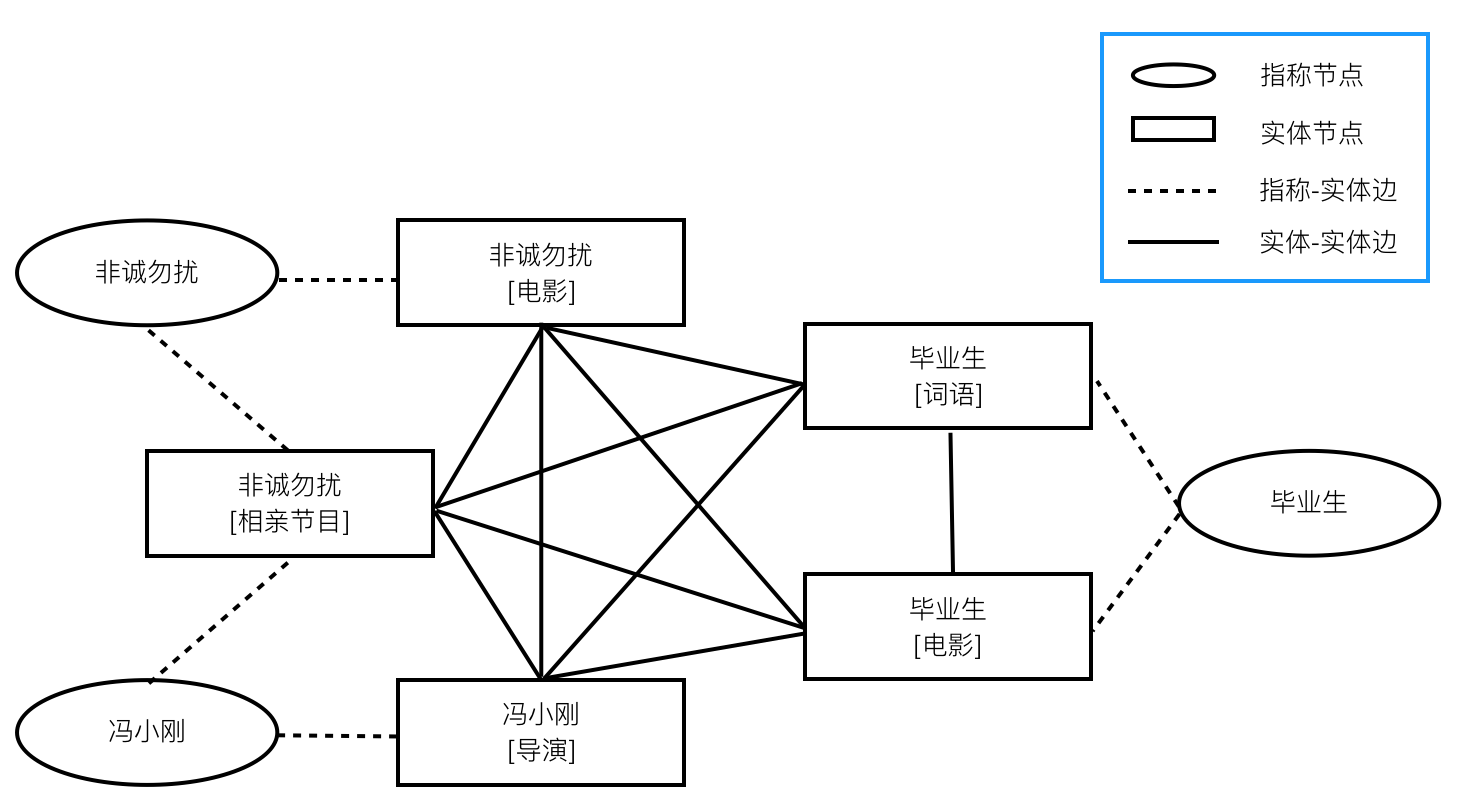
\includegraphics[width=0.9\textwidth]{img/edg}
\caption{一个构建好的实体消岐图示例}
\label{edg}
\end{figure}

b) \textbf{计算实体链接影响因子} \ 
在为给定的 Web 表格构建好实体消岐图之后,为每个结点和每条边上赋上一个概率值。
对于实体结点,结点上的概率表示它成为指称的对应参考实体的概率,在其被实体链接影响因子 (EL Impact Factors) 影响之前初始化为0。
实体链接影响因子实际上由2部分组成:
\begin{enumerate}[1)]
\item 指称结点的概率,它们代表了指称对于联合消岐的重要性
\item 边上的概率,即为结点间的语义相关度 (Semantic Relatedness)。
在本文中,认为每个指称都是地位平等的,所以当 Web 表格中有 k 个指称的时候,每个指称的重要性分值都初始化为 $\frac{1}{k}$。
因为在构建好的实体消岐图中有两种不同类型的边,指称-实体边与实体-实体边上的概率分别与指称-实体间的语义相关度和实体-实体间的语义相关度挂钩。
\end{enumerate}

对于\textbf{指称-实体间的语义相关度},我使用了两个特征来计算它,计算方式如下:
\begin{itemize}
	\item[$\bullet$] \textbf{字符串相似度特征} \ 
	假如一个指称 $m$ 和一个实体 $e$ 在字符串层面很相似,那么有可能 $e$ 是 $m$ 在给定知识库中的候选实体。
	因此,我把字符串相似度特征 $strSim(m,e)$ 定义为:
	\begin{equation}
	strSim(m,e)=1-\frac{Levenshtein(m,e)}{max\{|s|, |e|\}}
	\label{strsim}
	\end{equation}
	其中 $|m|$ 和 $|e|$ 分别是指称 $m$ 和实体 $e$ 的字符串长度。
	$Levenshtein(m,e)$ 代表 $|m|$ 和 $|e|$ 之间的莱文斯坦距离 (Levenshtein Distance\footnote{\url{https://en.wikipedia.org/wiki/Levenshtein_distance}}),是一个衡量两个字符串差异性的标准。
	如果指称 $m$ 和实体 $e$ 在字符串层面越相似,那么 $strSim(m,e)$ 的值会越高。
	\item[$\bullet$] \textbf{指称-实体的上下文相似度特征} \ 
	给定一个指称 $m$ 和其候选实体集合中的一个实体 $e$,假如两者是语义相关的,那么两者可能有相似的上下文 (Context)。
	在这里,为了获取给定指称 $m$ 的上下文,我先将 $m$ 所在的表格单元格的同行同列的其他单元格中的指称收集起来,然后再将这些收集到的指称分词,得到一个单词集合。
	我使用了当今顶级的中文分词工具``结巴中文分词\footnote{\url{https://github.com/fxsjy/jieba}}''来完成实验中的各种分词操作。
	最后,将这个单词集合中的所有单词作为 $m$ 的上下文并把它表示为 $menContext(m)$。
	对于实体 $e$ 的上下文,它来自知识库的两种类型的数据。
	一是知识库的信息盒属性 (Infobox Property)。
	打开任意一张知识库的实体页面,其中一般都会有一个包含实体的各种属性的表格,这就是信息盒。
	通过爬虫程序将知识库的所有的这种信息盒爬取下来,这就组成了信息盒属性数据,这些数据以 RDF\cite{munoz2014using} 三元组的格式存储,每个 RDF 三元组都由主语、谓语和宾语组成。
	我首先将所有包含实体 $e$ 的 RDF 三元组收集起来,如果 $e$ 在一个 RDF 三元组的主语中出现,那么将其宾语分词成一个单词集合。
	同理,如果 $e$ 在一个 RDF 三元组的宾语中出现,那么将其主语分词成一个单词集合。
	这样的单词集合是实体 $e$ 的上下文的一部分;
	二是知识库的摘要信息 (Abstract)。
	摘要信息一般位于知识库的实体页面的开头,是一个描述实体的段落。
	将知识库的所有的这种摘要信息爬取下来,就组成了摘要数据,这些数据同样是以 RDF 三元组的格式存储的,每个 RDF 三元组的主语是实体的名称,宾语是描述该实体的摘要。
	遍历知识库的整个摘要数据,将包含实体 $e$ 的 RDF 三元组收集起来,然后将这些三元组的宾语分词成一个单词集合。
	这样的单词集合构成了实体 $e$ 的上下文的另一部分。
	我用 $entContext(e)$ 来表示实体 $e$ 的上下文。
	为了计算指称 $m$ 和实体 $e$ 之间的指称-实体上下文相似度 $contSim_{me}(m,e)$,我应用了杰卡德相似度 (Jaccard Similaruty\footnote{\url{https://en.wikipedia.org/wiki/Jaccard_similarity}}),如下所示:
	\begin{equation}
	contSim_{me}(m,e)=\frac{|menContext(m)\bigcap{entContext(e)}|}{|menContext(m)\bigcup{entContext(e)}|}
	\end{equation}
\end{itemize}
对于给定的一个指称 $m$ 和一个实体 $e$,为了将二者之间的字符串相似度 $strSim(m,e)$ 和指称-实体上下文相似度 $contSim_{me}(m,e)$ 整合起来,我定义了如下公式所示的\textbf{指称-实体语义相关度} $SR_{me}(m,e)$:
\begin{equation}
SR_{me}(m,e)=c_1\times(\alpha_1 \cdot strSim(m,e) + \beta_1 \cdot contSim_{me}(m,e)) + c_2
\label{equation_srme}
\end{equation}
其中 $c_1$ 和 $c_2$ 是两个常量,在后面的迭代概率传播中的概率转移矩阵的计算中,需要保证实体消岐图的连通性,即边上的概率,或者说是结点间的语义相关度非零,所以为了保证指称 $m$ 和实体 $e$ 之间的语义相关度为非零,将 $c_1$ 和 $c_2$ 分别设为 0.99 和 0.01,这样 $SR_{me}(m,e)$ 至少为 0.01。
$\alpha_1$ 和 $\beta_1$ 分别是指称 $m$ 和实体 $e$ 之间的字符串相似度和指称-实体上下文相似度的权重值,在实验中,都设置为 0.5。
\newline

对于\textbf{实体-实体间的语义相关度},我也定义了如下两个特征来计算它:
\begin{itemize}
	\item[$\bullet$] \textbf{三元组关系特征} \ 
	本特征来自前面提到的知识库的信息盒属性数据,这些数据是以 RDF 三元组格式存储,每一条信息盒属性都是一个 RDF 三元组。
	如果两个实体处于同一个 RDF 三元组中,那么它们明显是语义相关的。
	因此,我用下面的公式来计算实体 $e_1$ 和实体 $e_2$ 之间的三元组关系特征 $IsRDF(e_1,e_2)$:
	\begin{equation}
  	IsRDF(e_1,e_2)=
  		\left\{ 
      	\begin{array}{l}
      	1,\ e_1\;and\;e_2\;are\;in\;the\;same\;RDF\;triple\\
      	0,\ otherwise
      \end{array} 
  	\right.
  	\end{equation}
    \item[$\bullet$] \textbf{实体-实体的上下文相似度特征} \ 
  	与指称-实体上下文相似度特征类似,语义相关的实体可能有相似的上下文。
  	使用与指称-实体上下文相似度特征中相同的办法来获取每个实体的上下文。
  	给定一个实体 $e_1$ 和一个实体 $e_2$,同样地我使用杰卡德相似度来计算两个实体的上下文 $entContext(e_1)$ 和 $entContext(e_2)$ 之间的实体-实体上下文相似度特征 $contSim_{ee}(e_1, e_2)$:
  	\begin{equation}
		contSim_{ee}(e_1,e_2)=\frac{|entContext(e_1)\bigcap{entContext(e_2)}|}{|entContext(e_1)\bigcup{entContext(e_2)}|}
	\label{contsim}
  	\end{equation}
\end{itemize}
为了获取实体 $e_1$ 和实体 $e_2$ 之间的语义相关度,我综合了三元组关系特征 $IsRDF(e_1,e_2)$ 和实体-实体上下文相似度特征 $contSim_{ee}(e_1, e_2)$ 来计算\textbf{实体-实体语义相关度},公式如下:
\begin{equation}
SR_{ee}(e_1,e_2)=c_3\times(\alpha_2 \cdot IsRDF(e_1,e_2) + \beta_2 \cdot contSim_{ee}(e_1,e_2)) + c_4
\label{equation_sree}
\end{equation}
其中 $c_3$ 和 $c_4$ 是两个常量,基于之前指称-实体语义相关度的计算中相同的原因,将 $c_3$ 和 $c_4$ 分别设为 0.99 和 0.01,这样 $SR_{ee}(e_1,e_2)$ 至少为 0.01。
$\alpha_2$ 和 $\beta_2$ 分别是实体 $e_1$ 和实体 $e_2$ 之间的三元组关系特征和实体-实体上下文相似度的权重值,在实验中,都设置为 0.5。
\newline

c) \textbf{迭代概率传播} \ 
为了将不同的实体链接影响因子 (EL Impact Factors) 结合起来,我使用了迭代概率传播这个随机游走算法来计算实体结点上的概率 (即为该实体成为给定指称的对应参考实体的概率) 直到收敛。
在每张实体消岐图上的迭代概率传播的具体过程在下一段中描述。\par

给定一张包含 $n$ 个结点 ($k$ 个指称结点和 $l$ 个实体结点) 的实体消岐图 $\bm{G}=(\bm{V},\bm{E})$,每个结点都被赋予了一个编号,所有结点编号范围为 $1 \sim n$。
$k$ 个指称结点意味着当前表格中的指称数量为 $k$,指称结点的编号范围为 $1 \sim k$,实体结点的编号范围为 $k+1 \sim n$。
我使用这些编号来代表结点,并且用 $\bm{A}$ 来表示实体消岐图 $\bm{G}$ 的 $n \times n$ 的邻接矩阵,$\bm{A}_{ij}$ 指的是结点 $i$ 到结点 $j$ 的转移概率。
换句话说,矩阵 $\bm{A}$ 就是实体消岐图这个马尔科夫链模型的概率转移矩阵 (Transition Matrix)。
正如在构建实体消岐图一节中提到的,实体消岐图是一个无向带权图,同时也可以认为是一个双向图,因此结点 $i$ 与结点 $j$ 之间存在两个转移概率,一个是从结点 $i$ 到结点 $j$ 的转移概率,另一个是从结点 $j$ 到结点 $i$ 的转移概率。
鉴于结点 $i$ 到结点 $j$ 的边上已经被赋予了一个概率值,其表示不同结点间的语义相关度 (在公式~\ref{equation_srme} 和公式~\ref{equation_sree} 中定义),我将 $\bm{A}_{ij}$ 定义为:
\begin{equation}
\bm{A}_{ij}=\left\{
\begin{array}{rcl}
\frac{SR_{me}(i,j)}{SR_{me}(i,*)} && {if \ i \neq j,\ i\ is\ a\ mention\ node\ and\ j\ is\ an\ entity\ node}\\
(1-SR_{em}(i)) \times \frac{SR_{ee}(i,j)}{SR_{ee}(i,*)} && {if\ i \neq j,\ i\ and\ j\ are\ two\ entity\ nodes}\\
\frac{SR_{me}(j,i)}{SR_{me}(j,*)} && {if \ i \neq j,\ i\ is\ an\ entity\ node\ and\ j\ is\ a\ mention\ node}\\
0 && {otherwise}
\end{array} \right.
\label{aij}
\end{equation}
其中 $SR_{me}(i, j)$ 是一个指称结点 $i$ 和一个实体结点 $j$ 间的指称-实体语义相关度 (在公式~\ref{equation_srme} 中定义)。
$SR_{ee}(i, j)$ 是一个实体结点 $i$ 和一个实体结点 $j$ 之间的实体-实体语义相关度 (在公式~\ref{equation_sree} 中定义)。
$SR_{ee}(i, \ast)$ 指的是实体结点 $i$ 与其相邻的所有实体结点间的实体-实体语义相关度的总和。
$SR_{me}(i, \ast)$ 指的是指称结点 $i$ 与其相邻的所有实体结点间的指称-实体语义相关度的总和。
$SR_{em}(i)$ 指的是实体结点 $i$ 与其唯一相邻的指称结点间的指称-实体语义相关度。\par

最后,我给实体消岐图中的所有结点定义了一个 $n \times 1$ 的一维矩阵 $\bm{r}$,$\bm{r}(i)$ 表示结点 $i$ 成为某指称的对应参考实体的概率 (假如 $i$ 是一个实体结点)。
$\bm{r}$ 的计算就是迭代概率传播的过程,首先将整个一维矩阵初始化为 $\bm{r}^0$。
就像前面介绍的那样,如果结点 $i$ 是一个指称结点,那么 $\bm{r}^0(i)$ 设为 $i$ 的初始重要性分值,也就是 $\frac{1}{k}$。
假如结点 $i$ 是一个实体结点,那么 $\bm{r}^0(i)=0$。
然后,使用其他实体链接影响因子,也就是矩阵 $\bm{A}$ 中编码的指称-实体语义相关度和实体-实体语义相关度,在迭代概率传播的过程中不断更新 $\bm{r}$。
通过这样的方式,$\bm{r}$ 的递归形式如下所示:
\begin{equation}
\bm{r}^{t+1}=((1-d) \times \frac{\bm{E}}{n} + d \times \bm{A}) \times \bm{r}^t
\label{r}
\end{equation}
其中 $t$ 是迭代的轮数,鉴于有时 $\bm{r}$ 收敛 (每个实体结点上的概率都收敛) 得很慢,我设置了一个迭代次数的上限 $limit$,当迭代次数超过了该上限而矩阵还未收敛,则停止迭代。
$\bm{E}$ 是一个 $n \times n$ 的单位阵,即其中所有元素都是 1。
在公式~\ref{r} 中,为了确保概率转移矩阵 $\bm{A}$ 的不可约性 (Irreducible) 和非周期性 (Aperiodic) 从而使实体结点上的概率值能够收敛,又因为每一个元素都为正的概率转移矩阵是不可约和非周期的\cite{tauchen1986finite},我给实体消岐图中的任意两个结点之间加了一种特殊类型的无向边,并且给这样的每条边上赋予一个很小的转移概率,这个转移概率由衰减系数 $d$ 控制。
换句话说,在迭代概率消岐的过程中,存在一种可能性在于实体链接影响因子的传播既不通过先前定义的指称-实体边也不通过实体-实体边,而是通过上面那种特殊类型的带很小转移概率的边。
因为迭代概率传播的过程与 PageRank\cite{page1999pagerank} 算法很相似,所以我把衰减系数同样设置为 0.85。
在迭代概率传播之后,给定一个指称 $m$ 和它的候选实体集合 $Candidate(m)=\{e_1, e_2, ..., e_s\}$,挑选其中概率值最高的实体作为 $m$ 的对应参考实体。\par

与其他方法不同的是,上述的单知识库表格实体链接算法不依赖与任何特定的信息,只基于知识库的各种类型的通用数据 (RDF 三元组)。
因此它可以被应用于任何包含开放链接数据\footnote{\url{http://linkeddata.org/}} (Linking Open Data) 中 RDF 三元组数据的知识库,比如 YAGO\cite{suchanek2007yago},DBpedia\cite{auer2007dbpedia},Freebase\cite{bollacker2008freebase},Zhishi.me\cite{niu2011zhishi}等。


\subsection{多知识库提升链接结果}\label{multiple}

只用单知识库进行表格的实体链接因为单知识库的实体缺失问题不能总是保证一个很好的覆盖程度 (Coverage)。
这个问题的一个解决方案是用不同的知识库分别进行实体链接的任务,来提高实体链接结果的覆盖程度。
然而,这样又可能会导致不同知识库下的实体链接结果的冲突。
在本文中,我在 Zhishi.me 上进行了~\ref{approach1} 节中描述的方法一的测试实验。
如图~\ref{zhishime_data} 中所示,Zhishi.me 包含了三个最大的中文在线链接百科知识库:中文维基百科,百度百科和互动百科。
我首先将上述单知识库实体链接方法应用于从中文维基百科、百度百科和互动百科上抽取出的 Web 表格 (超过7万张)。
然后,给定一张 Web 表格中的一个指称 $m$ 和其在三个知识库中识别出的参考实体 $\{e_1(zhwiki), e_2(baidubaike), e_3(hudongbaike)\}$。
假如两个来自不同知识库的实体之间存在``sameAs''关系,那么它们是等价的,可以看成是相同的实体,否则它们是不同的实体。
假设三个参考实体间不存在``sameAs''关系,就意味着此时指称 $m$ 链接到了三个不同的实体上。
也就是说,指称 $m$ 的链接结果存在冲突。图~\ref{sameas} 中就是一个链接冲突的例子。
根据数据统计,大约有 38.94\% 的实体链接结果 (一个结果指的是一个指称与其在不同知识库中识别出的实体) 存在冲突。
我观察了上述测试实验的实体链接结果以及分析了这些使用不同知识库进行实体链接结果产生冲突的原因。
有以下两点原因:
\begin{itemize}
  \item[$\bullet$] \textbf{原因一}: 对于一些知识库,某些实体链接的结果实在是不正确的,这就造成了一些潜在的正确的参考实体并没有在指称的候选实体集合中排名最高。
  \item[$\bullet$] \textbf{原因二}: 知识库间的``sameAs''关系是不完整的,一些来自不同知识库的等价实体间并没有``sameAs''关系标记。
\end{itemize}
基于这两个原因,我在接下里的部分会详细介绍解决多知识库实体链接冲突的方法。\par

% Fig 
\begin{figure}[htbp]
\centering
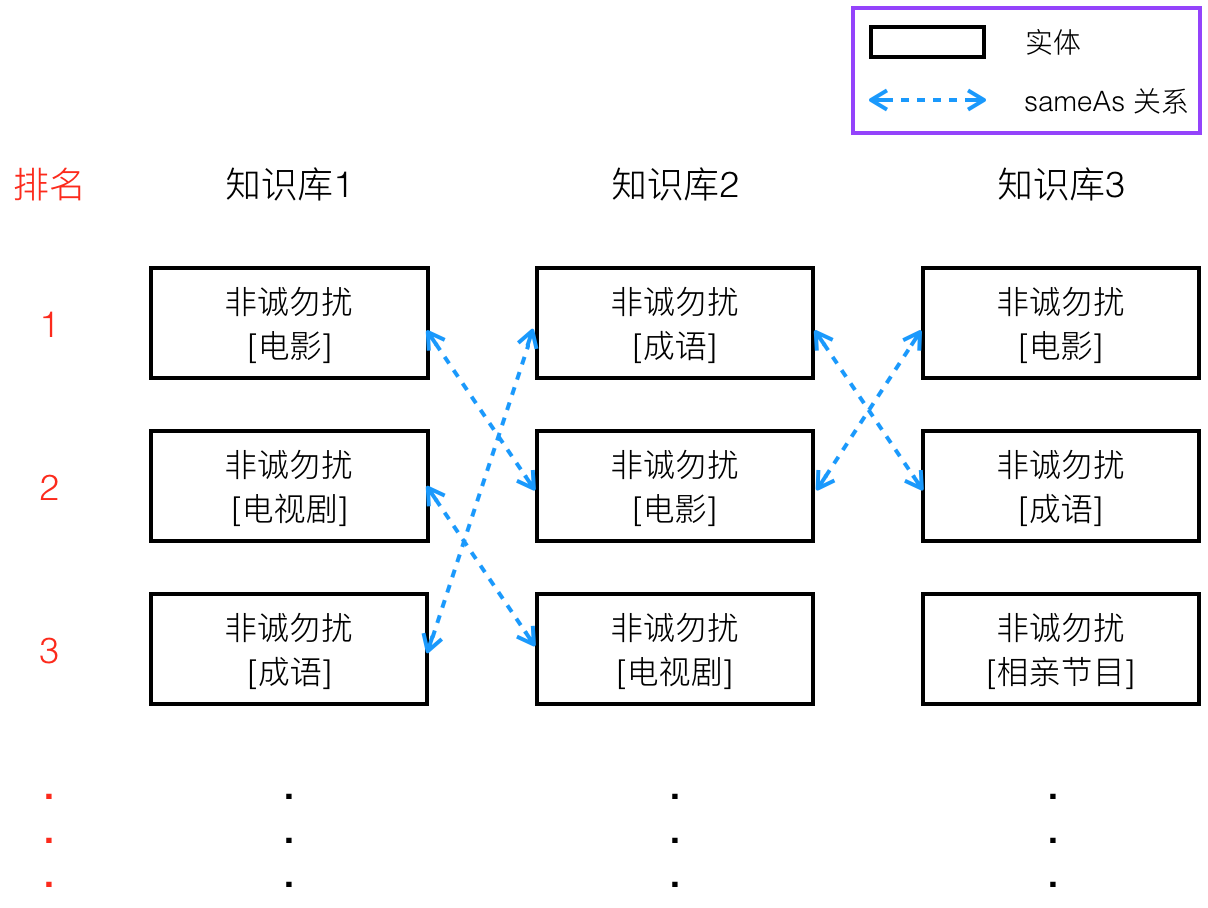
\includegraphics[width=0.8\textwidth]{img/sameas}
\caption{一个实体链接结果的实例:图~\ref{table} 中指称``非诚勿扰''在不同知识库上的候选实体的排名列表}
\label{sameas}
\end{figure}

假定有 $n$ 个不同的相互链接的知识库,两个知识库相互链接指的是二者的实体由``sameAs''关系相互关联。
对每个给定的知识库,我先使用~\ref{single} 节中提出的方法进行 Web 表格的单知识库实体链接。
对于每个指称,能够得到它的前 $n$ 个候选实体排名列表。
然后,利用不同知识库实体间的``sameAs''关系,我将候选实体排名列表中等价的实体分到一组,最后所有实体分成多个不同的组,每个组中的实体都是``sameAs''的。
例如,在图~\ref{sameas} 中,我能够得到如下的四组实体:
\begin{enumerate}[1)]
\item $Set_1=$ \{``非诚勿扰[电影]'' ($KB_1$), ``非诚勿扰[电影]'' ($KB_2$), ``非诚勿扰[电影]'' ($KB_3$)\}
\item $Set_2=$ \{``非诚勿扰[成语]'' ($KB_1$), ``非诚勿扰[成语]'' ($KB_2$), ``非诚勿扰[成语]'' ($KB_3$)\}
\item $Set_3=$ \{``非诚勿扰[电视剧]'' ($KB_1$), ``非诚勿扰[电视剧]'' ($KB_2$)\}
\item $Set_4=$ \{``非诚勿扰[相亲节目]'' ($KB_3$)\}
\end{enumerate}
有了分好组的实体的之后,计算每组实体的平均排名、最高排名和组内实体数量。
举个例子,对于 $Set_1$ 中的实体,平均排名就是 $\frac{1+2+1}{3}=1.33$,最高排名是 1,实体数量为 3。
最后,我提出了三条启发式的规则来解决多知识库实体冲突的问题,并选择一个实体分组作为给定指称的最终实体链接结果。
\begin{itemize}
  \item[$\bullet$] \textbf{规则一}: 如果一个实体分组的平均排名、最高排名在所有分组中排名最高,并且该组的实体数量不少于知识库数量的一半,那么选择这一组作为给定指称的最终实体链接结果。
  \item[$\bullet$] \textbf{规则二}: 如果有两个或多个实体分组的平均排名、最高排名相同并在所有分组中排名最高,并且这些分组的实体数量不少于知识库数量的一半,那么从这些分组中随机挑选一组作为给定指称的最终实体链接结果。
  \item[$\bullet$] \textbf{规则三}: 如果每组的实体数量都小于知识库数量的一半,那么对于给定指称,原先单知识库实体链接结果保持不变。
\end{itemize}
为了同时获得全局和局部最优的实体链接结果,我不光考虑了每个实体分组的平均排名和最高排名,还考虑每个个体 (由一个实体分组表示) 在不同知识库中的出现次数。
如果一个实体分组中的实体数量小于知识库数量的一半,这意味着这组实体表示的个体被很少的知识库所覆盖,所以平均排名并不具有说服力,也没有理由选择这个实体分组来解决多知识库的实体链接结果冲突问题。


\section{方法二: 融合}\label{approach2}
方法二尝试将方法一中的两步合并为一步,用一个统一的图模型来表示表格指称和来自多知识库的其候选实体以及实体间的``sameAs''关系。
方法二的流程与方法一无异,依旧先是指称识别,然后候选实体生成,最后实体消岐,实体消岐分为三个小步骤:构建实体消岐图,计算实体链接影响因子和迭代概率传播。
在本文中,二个方法进行指称识别和候选实体生成的方式是完全相同的,它们使用的输入数据 (表格,多知识库的各类型数据) 也是相同的。
方法二与~\ref{approach1} 节中描述的方法一的区别主要在于实体消岐图中结点定义的改变以及舍弃了~\ref{multiple} 节中提到的三条启发式规则。
在这里,我重新给出实体消岐图的定义。
\begin{itemize}
  \item[$\bullet$] \textbf{指称结点}: 这些结点指的是 Web 表格中的字符串指称
  \item[$\bullet$] \textbf{实体组结点}: 这些结点表示指称在多知识库中的基于``sameAs''的所有候选参考实体
  \item[$\bullet$] \textbf{指称-实体组边}: 一条指称-实体组边是一个指称和其候选参考实体组集合中的一个实体组之间的无向边
  \item[$\bullet$] \textbf{实体组-实体组边}: 一条实体组-实体组边是实体组之间的无向边
\end{itemize}
将方法一中提到的实体消岐图中的实体结点转变为实体组结点。
原先的实体结点只包含了一个实体,而且一张实体消岐图中所有实体结点都来自同一个知识库。
如图~\ref{edg2} 中那样,现在的实体组结点包含了一个或者多个实体,利用多知识库实体间的``sameAs''关系,将有``sameAs''关系的来自不同知识库的实体放入同一个结点,即实体组结点。
这样就将多知识库实体间的``sameAs''关系融合进实体消岐图模型了。
这种融合让我有机会实现原先方法中两步的合并。

\begin{figure}[htbp]
\centering
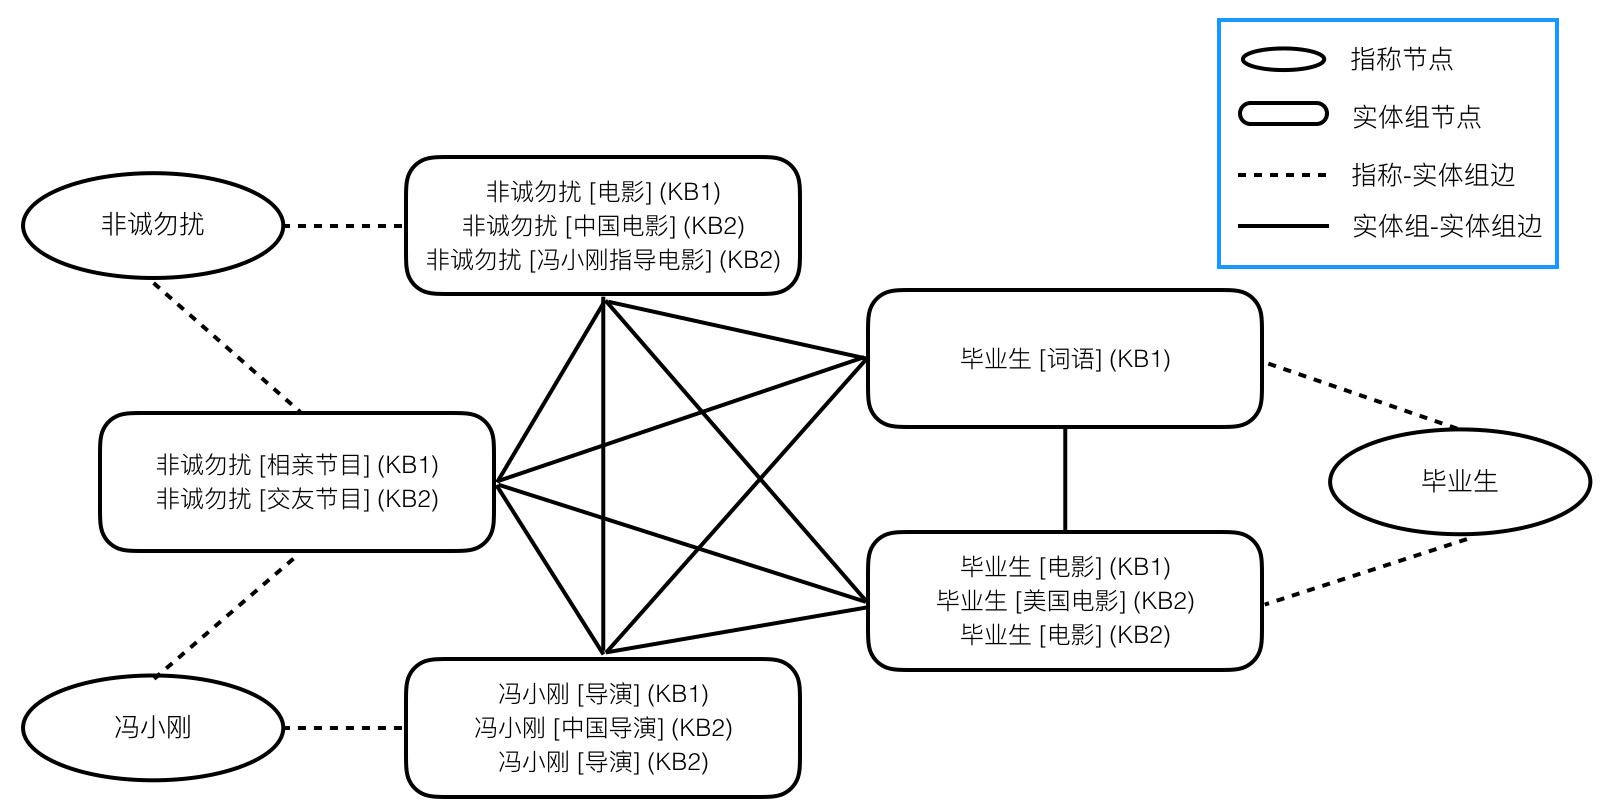
\includegraphics[width=0.9\textwidth]{img/edg2}
\caption{一个构建好的新实体消岐图示例}
\label{edg2}
\end{figure}

构建好实体消岐图之后,接着计算实体链接影响因子。
在计算一个指称 $m$ 与一个实体组 $entitySet=\{e_1 (kb1), e_2 (kb2), e_3 (kb3)\}$ 之间的\textbf{指称-实体组语义相关度}的时候,我采用的是分别计算指称 $m$ 与实体组 $entitySet$ 中每个实体的\textbf{指称-实体语义相关度},然后取平均值作为指称 $m$ 与实体组 $entitySet$ 的\textbf{指称-实体组语义相关度}。
同样的,在计算一个实体组 $entitySet1$ 与一个实体组 $entitySet2$ 之间的\textbf{实体组-实体组语义相关度}的时候,分别计算实体组 $entitySet1$ 中每个实体与实体组 $entitySet2$ 中每个实体的\textbf{实体-实体语义相关度},然后取平均值作为实体组 $entitySet1$ 与实体组 $entitySet2$ 之间的\textbf{实体组-实体组语义相关度}。
最后,在构建好的实体消岐图上,结合实体链接影响因子,使用 \ref{single} 中相同的迭代概率传播方式在实体消岐图上进行随机游走算法,得到给定指称在多知识库中的对应参考实体组作为最终的实体链接结果。


\section{sameAs 关系的学习}
在~\ref{multiple} 节中我提到导致多知识库实体链接结果冲突的一个重要原因就是``sameAs''关系的缺失。
如果不同知识库的实体间能够存在更多的``sameAs''关系,这种冲突问题可能能够被更好的解决。
为了能够学习到新的``sameAs''关系,我定义了三个特征并训练了一个监督学习分类器支持向量机\cite{tong2001support} (Support Vector Machine),其在大多数情况下\cite{fernandez2014we}有着最好的性能表现。
三个特征在下面介绍:
\begin{itemize}
  \item[$\bullet$] \textbf{同义词特征}: 这个特征用于检测两个实体字符串是否是同义词。我将两个实体字符串 $e_1$ 和 $e_2$ 输入进 BabelNet\cite{navigli2010babelnet},如果在 BabelNet 中这两个字符串有同义词关系,那么同义词特征 $isSyn = 1$,否则 $isSyn = 0$。
  \item[$\bullet$] \textbf{字符串相似度特征}: 这个特征捕捉实体间的语言学上的相关性 (Linguistic Relatedness)。两个实体 $e_1$ 和 $e_2$ 之间的字符串相似度由 $strSim(e_1, e_1)$ 表示。我使用公式~\ref{strsim} 来计算它。
  \item[$\bullet$] \textbf{实体-实体上下文相似度特征}: 对于两个来自不同知识库的实体,这个特征捕捉实体的上下文之间的相似度并且已经在公式~\ref{contsim} 中定义
\end{itemize}
除了使用支持向量机分类器来学习新的``sameAs''关系,我还考虑使用实体链接与``sameAs''进行迭代学习。
如果在最终的实体链接结果中,两个来自不同知识库的实体被同一个指称链接到,但这两个实体间并没有``sameAs''关系标记,那么此时可以为这两个实体添加``sameAs''关系。
这样就学到了新的``sameAs''关系。
而``sameAs''关系反过来又能促进实体链接,换句话说,实体链接与``sameAs''关系的学习是相互促进的。
因此让它们迭代学习既能补全多知识库间的``sameAs''关系,又能提升实体链接的质量。


\section{本章小结}
在这一章中,我首先介绍了实体链接方法中用到的两个模型:马尔科夫链模型和随机游走模型。
然后详细描述了本文提出的两个方法。
这两个方法是平行的,方法一是一个两阶段的方法,方法二是方法一的改版,其融合了方法一中的两步,这两个方法的输入和输出都是一样的。
输入都是 Web 表格和多知识库的实体数据,输出都是表格的实体链接结果,即表格中的字符串指称最终链接到的知识库中对应的参考实体。
换句话说,这两个方法中的任何一个都可以单独拿出来作为一个表格实体链接系统的核心算法。
目前实体链接的方法大体上可以分为3类:基于概率统计的方法,基于机器学习的方法和基于图模型的随机游走方法。
本文中的两个方法的核心都是属于基于图模型的随机游走方法。
这类方法的思路与另外2类方法完全不同。
它主要利用字符串指称与实体之间、实体与实体之间的语义相关性来开展实体链接的工作。


\chapter{系统实现}

\section{表格语料库}

\section{知识库实体}

\section{人工标注指称来源}

\section{本章小结}

\chapter{实验与评估}
在本章中,我使用 Zhishi.me 中的三个相互链接的知识库 (中文维基百科,百度百科和互动百科) 评估了系统中的方法。
整个评估过程基于人工标注的 Web 表格。
并且将系统中的方法与两个先进的 Web 表格实体链接系统以及我的方法的两个退化版本 (Degenerate Version) 进行比较。

\section{评价标准}
我在每张人工标注过的 Web 表格上使用系统中的方法进行实体链接并用设计好的对比实验进行对比。
在实验中,使用了四个指标 (Metric) 来衡量链接结果的质量。
它们分别是准确率 (Precision),召回率 (Recall),F1值 (F1-score) 和 平均倒数排名 (Mean Reciprocal Rank\cite{craswell2009mean}, MRR)。
这些评价指标普遍用于文本的实体链接任务\cite{bhagavatula2015tabel}。
F1值是准确率和召回率的调和平均数。
平均倒数排名 (MRR) 用来评估指称的候选实体排名列表的质量。
对于一个指称 $m$,实体链接的倒数排名 (Reciprocal Rank) 是 $m$ 的正确参考实体在候选排名列表中的排名的倒数。
比如,$m$ 的正确参考实体在由实体链接算法生成的候选实体排名列表中排在第二位,则倒数排名为 $\frac{1}{2}$。


\section{几种方法的比较}
我对以下方法进行了对比试验。

\begin{itemize}
  \item[$\bullet$] $TabEL$: TabEL\cite{bhagavatula2015tabel} 是目前 Web 表格实体链接领域先进的系统,它使用一种使用了许多通用特征的集体分类技术来对一个给定 Web 表格中的所有指称进行联合消岐。除此之外,任何知识库都可以被应用于 TabEL 来执行 Web 表格上的实体链接任务。
  \item[$\bullet$] $LIEGE$: LIEGE\cite{shen2012liege} 是一个通用方法,用于将形如列表 (List-like) 的 Web 表格 (多行一列) 中的字符串指称链接到给定知识库中的参考实体。它提出了一种使用了三个特征的迭代置换算法来执行 Web 列表中的实体链接。这个方法同样可以用于任何知识库上的 Web 表格实体链接。
  \item[$\bullet$] $single$: 是 $approach1$ 的一个退化版本。它只使用了方法一中单知识库实体链接的算法,并没有运用三条启发式规则和``sameAs''关系来执行多知识库对实体链接结果的优化算法。
  \item[$\bullet$] $multiple$: 也是 $approach1$ 的一个退化版本。在执行完单知识库实体链接算法后,它仅使用了已存在的``sameAs''关系 (不包括新学习到的``sameAs''关系) 来提升实体链接结果质量。
  \item[$\bullet$] $approach1$: 即为~\ref{approach1} 节描述的方法一。它分为两步,先用每个单知识库进行实体链接,然后用多知识库间的``sameAs''关系进行链接结果的优化。它采用了一种基于图的随机游走算法来实现一个表格中所有指称的联合消岐。同样,它也是一个通用算法,任何拥有丰富 RDF 三元组格式数据的知识库都可以作为该方法的输入。
  \item[$\bullet$] $approach2$: 即为~\ref{approach2} 节描述的方法二。它融合了方法一中的两步,使用了一个统一的图模型来表示一个给定表格的所有指称和候选实体以及多知识库间的``sameAs''关系。它也是一个适用于任何知识库的多知识库实体链接算法。
\end{itemize}

% Table
\begin{table}[htbp]
\centering
\caption{由三个单知识库衡量的总体实体链接结果}
\label{result}
\begin{tabular}{|c|c|c|c|c|c|}
\hline
Knowledge Base & Approach & Precision & Recall & F1-score & MRR \\
\hline
\multirow{6}{*}{Chinese Wikipedia} & TabEL & 0.823 & 0.809 & 0.816 & 0.858 \\
\cline{2-6} & LIEGE & 0.778 & 0.747 & 0.762 & 0.813 \\
\cline{2-6} & single & 0.830 & 0.797 & 0.813 & 0.860 \\
\cline{2-6} & multiple & 0.861 & 0.821 & 0.841 & 0.881 \\
\cline{2-6} & approach1 & \textbf{0.873} & \textbf{0.828} & \textbf{0.850} & \textbf{0.887} \\
\cline{2-6} & approach2 & \textbf{0.856} & \textbf{0.830} & \textbf{0.843} & \textbf{0.814} \\
\hline
\multirow{6}{*}{Baidu Baike} & TabEL & 0.659 & 0.628 & 0.643 & 0.707 \\
\cline{2-6} & LIEGE & 0.629 & 0.576 & 0.601 & 0.670 \\
\cline{2-6} & single & 0.696 & 0.652 & 0.673 & 0.725 \\
\cline{2-6} & multiple & 0.758 & 0.705 & 0.731 & 0.746 \\
\cline{2-6} & approach1 & \textbf{0.774} & \textbf{0.727} & \textbf{0.750} & \textbf{0.776} \\
\cline{2-6} & approach2 & \textbf{0.769} & \textbf{0.747} & \textbf{0.758} & \textbf{0.780} \\
\hline
\multirow{6}{*}{Hudong Baike} & TabEL & 0.681 & 0.649 & 0.665 & 0.780 \\
\cline{2-6} & LIEGE & 0.661 & 0.632 & 0.646 & 0.751 \\
\cline{2-6} & single & 0.708 & 0.642 & 0.673 & 0.768 \\
\cline{2-6} & multiple & 0.729 & 0.700 & 0.714 & 0.787 \\
\cline{2-6} & approach1 & \textbf{0.744} & \textbf{0.708} & \textbf{0.726} & \textbf{0.796} \\
\cline{2-6} & approach2 & \textbf{0.731} & \textbf{0.712} & \textbf{0.721} & \textbf{0.788} \\
\hline
\end{tabular}
\end{table}


\section{结果分析}
表格~\ref{result} 给出了系统中两个实体链接方法的总体结果和由三个单知识库分别衡量的对比实验的结果,从中我可以发现:
\begin{itemize}
  \item[$\bullet$] 方法一中的单知识库实体链接方法,也就是 $single$,其效果能够与当前非常先进的实体链接系统 TabEL 相媲美,并且胜过 LIEGE。这反应了我在系统中提出的方法的有效性。
  \item[$\bullet$] $multiple$ 方法在准确率、召回率、F1值和 MRR 上总是比 $single$ 方法更好。这表明方法一中提出的启发式规则在提升单知识库实体链接结果上是非常有价值的。
  \item[$\bullet$] 系统中的方法一,也就是 $approach1$,在准确率这个指标上比其他所有对比方法都高,这证实了方法一在多知识库 Web 表格实体链接上的优越性。与 $multiple$ 方法相比,方法一具有更好的表现,这体现了新学习到的``sameAs''关系对于解决用不同知识库进行单知识库实体链接 ($single$) 导致的链接冲突问题是很有帮助的。
  \item[$\bullet$] 系统中的方法二,也就是 $approach2$,在准确率这个指标上仅次于方法一,这体现出方法二也是非常有效的。而且与 $approach1$ 相比,$approach2$ 在召回率这个指标上表现更佳,这说明方法一中的启发式规则由于不稳定性导致没有覆盖到一些正确的参考实体,而方法二弥补了这一点。
\end{itemize}
另外,我用整个 Zhishi.me 来衡量的方法一 ($approach1$) 的实体链接结果,并计算了准确率、召回率、F1值。
准确率是0.831,召回率是\textbf{0.903},F1值为0.866。
可以发现召回率有了显著的提升,这表明多知识库的表格实体链接方法的确能够保证一个很好的实体覆盖度。


\section{本章小结}
本章首先介绍了对比试验的评价指标:准确率、召回率、F1值和 MRR。这些都是常见的实体链接算法的评价指标。
然后描述了我设计的六组对比试验,并以表格的形式给出了对比结果。
最后对实体链接的结果进行了对比分析,试验结果表明系统中的多知识库表格实体链接方法的有效性并且相对于单知识库实体链接能够有一个更好的实体覆盖度。
\chapter{总结与展望}

\section{工作总结}
在这篇论文中,我提出了两个新的基于多知识库的表格实体链接方法。
两个方法的核心都是基于图的随机游走算法。
方法一的第一步是用一个基于图的迭代概率传播算法来进行单知识库实体链接。
在第二步中我提出了三条启发式规则来利用不同知识库实体间的``sameAs''关系来提升第一步的链接结果,同时也解决了多知识库实体链接结果冲突的问题。
方法二中使用了一个统一的图模型,直接将多知识库的实体和实体间的``sameAs''关系融合进实体消岐图,一步到位地计算出实体链接结果。
两个方法都有各自的优缺点。
优点在于二者都不依赖特定的信息 (表格的列头,知识库中的实体类型),
并且都是基于多知识库进行实体链接,弥补了单知识库实体覆盖程度不够的缺点。
方法一的缺点在于其第二步中的启发式规则的不稳定性。
方法二的缺点在于,在构建实体消岐图的时候,很多正确的参考实体由于``sameAs''关系缺失的原因不能和其他等价的实体进入同一个实体组结点,又因为链接的目标是为一个给定的指称选择一个实体组结点作为链接结果,作为这样就导致了最终链接结果会有所遗漏。
我设计并实现了两个方法与 TabEL\cite{bhagavatula2015tabel},LIEGE\cite{shen2012liege} 以及另外两个退化版本的方法的对比实验。
实验结果表明本文中的两个方法在不同的评价标准 (准确率、召回率、F1值和 MRR) 上表现得都非常优秀。
并且这两个多知识库表格实体链接方法都非常有效并且相对于单知识库实体链接有一个更好的实体覆盖度。
值得一提的是,本文中的两个方法都是通用的,可以使用任何单知识库或者相互链接的多知识库进行 Web 表格上的实体链接。


\section{未来展望}
在~\ref{challenge} 节中提到当前实体链接的关键挑战在于缺少基准数据集。
因此对于未来的工作,首要任务是建立更多的其他语言的基准数据集,用于开展基于多知识库的 Web 表格实体链接的新任务。
其次是改进优化本文中提出的方法,比如在计算实体链接影响因子的时候设计更多的特征,原先使用的特征主要反映的是指称与实体之间、实体与实体之间的语义相关度,更多有效特征的加入可以多维度地反映指称与实体之间、实体与实体之间的关系,从而提升链接的质量。
更进一步地,衡量本文中的方法在其他语言上,特别是英语上的效果。
除此之外,我还考虑加上关系抽取的功能。
就像~\ref{task} 节中提到的,关系抽取是表格语义解释的主要任务之一。
根据表格中不同列实体链接的结果,通过两列某一行的关系即可得到表格列之间的关系,最终的结果表示为 RDF 三元组。
然后,我计划把本文中的方法进行封装,做成编程接口,提供 API 或者工具供他人使用,或者将这些接口做成 Web 应用,让他人通过 Web 就能轻松使用我的方法进行实体链接。
最后,我考虑将上述方法拓展成跨语言\cite{zhang2013cross} (Cross-lingual) 的多知识库表格实体链接方法。









\end{Main}
% 结束正文

% 致谢
\begin{Acknowledgement}
在这篇本科毕业论文撰写的过程中,很多人帮助了我,在此我向他们致以我最高的敬意。\par

首先是我的家人,是你们的支持,让我能够顺利完成学业,成为一个有独立思想的人。

我要感谢我的导师漆桂林教授。
从我大二开始,他就悉心地指导我进行数据挖掘和实体链接方面的学习和研究。
在我大三那年,我和计算机学院的另外四名同学一起在他的指导下开展了 SRTP 项目``基于社交数据的实体链接研究''并最终取得了丰厚的成果。
在我的毕业设计中,他给出了许多建设性意见来启发我。
漆老师是学术上的导师,也是人生上的导师,他严谨的科研态度和务实的精神一直影响着我。
不管是在生活中还是在学习中,他都给我提供了很多帮助。
在此,我要对他表示我的尊敬之情与感谢之意!\par

我要感谢我的毕设导师李慧颖教授。
她耐心细致的教导为我的毕业设计保驾护航。\par

我要感谢我的师兄吴天星博士和刘太云学长。
是他们不断地督促我开展科研和学习新知,是他们在我遇到问题的时候耐心回答我的疑问,是他们的创造力不断启发着我。
与吴天星博士每周一次的讨论给我带来了很多科研上的新思路新方法。
没有他们的指导和帮助,我的毕设不可能顺利地完成。
同时我还要感谢知识科学与工程实验室,感谢实验室给我带来的经历与帮助。\par

我要感谢我的4位同学许亮、朴智新、王瑞明和段尚甫。
在大学四年时间里,我们互相关照共同进步,一起留下了许多珍贵而美好的记忆。
在大三的 SRTP 项目中,我们就并肩作战,共同实现项目的各类算法和实验。
是他们的才智与能力让项目中实体链接的研究开展得高效顺利。
他们也为我的毕设提供了很多技术上的帮助与建议。\par

我要感谢计算机科学与工程学院。
学院给我提供了一个优质的平台来自我成长,学院丰富的教学资源让我受益颇丰。
此外,我要感谢学院里一直默默为学生付出的工作人员,比如吕倩老师和洪小丽老师。
她们给我的学习和生活上提供了很多的便利。\par

在东南大学的四年,可能是我人生中最美妙的四年。
我在这里学到了很多,成长了很多,也认识了许多卓越的老师和同学。
这都会是我人生中最宝贵的精神财富。
本科毕业论文意味着大学四年的结束,也代表着一个新的开始。
是时候跟美好的大学生活说再见了,是时候去勇敢地拥抱新生活了!\par

最后,谨以此文献给我的母亲沈芳。
\end{Acknowledgement}

% 参考文献
\bibliography{seuthesis}

% \begin{Appendix}
%   \chapter{附录}
%   附录
% \end{Appendix}

\newpage
\printindex % 索引

% \begin{thebibliography}{99}
% \bibliographystyle{spmpsci}
% \bibliography{seuthesis}

% 作者简历
% \begin{Resume}
% 作者简介
% \end{Resume}

\end{document}